\chapter{Annotation Continuum} % Main chapter title
\label{ch:annotation} % Change X to a consecutive number; for referencing this chapter elsewhere, use \ref{ChapterX}

This chapter studies the social AR continuum in term of interactions between users. The interaction is represented by adding an AR tag or annotation on a shared medium to socially connect with other users. 
The aim of this chapter is to answer the research question RQ2: "How to represent annotations/tags on shared social experience through wearable AR devices"
The first section \ref{sec:video} addresses annotation on a live video stream. The second section \ref{sec:3D} studies the annotation on a 3D environment using 3D sensors to detect the shared surrounding environment. 


\section{AR Annotation on Social Video Sharing}
\label{sec:video}
% =============== PREVIOUS WORK ================

% A. Nassani, H. Kim, G. Lee, M. Billinghurst, T. Langlotz, and R. W. Lindeman, “Augmented reality annotation for social video sharing,” in SIGGRAPH ASIA 2016 Mobile Graphics and Interactive Applications on - SA '16, 2016, pp. 1–5.

% =============== PREVIOUS WORK ================


% \subsection{Abstract}

This paper explores different visual interfaces for sharing comments on a social live video streaming platforms. So far, comments are displayed separately from the video making it hard to relate the comments to event in the video. In this work we investigate an Augmented Reality (AR) interface displaying comments directly on the streamed live video. Our described prototype allows remote spectators to perceive the streamed live video with different interfaces for displaying the comments. We conducted a user study to compare different ways of visualising comments and found that users prefer having comments in the AR view rather than on a separate list. We discuss the implications of this research and directions for future work.

% \subsection{Introduction}

% Advancements in mobile phone hardware and increased network connectivity made live video streaming apps popular among smart phone users. Live video streaming apps have been used for sharing social experiences in various contexts. For instance, a person attending a conference or a concert could use her mobile phone to stream the event to her friends and family who could not be there. Similarly, live video streaming apps have also been used for Social journalism turning laypersons into live reporters. Consequently, these apps are now available from different sources with applications such as Periscope\footnote{https://www.periscope.tv/} and Facebook Live\footnote{https://live.fb.com/} among the most popular apps. 

% They all share common features such as using the phones' camera which can be either pointed outward (recording what the user sees) or inward (where the user appears in the video) and allowing users to send a live video stream of what they are doing to hundreds or even thousands of viewers. The purpose of sharing the video is social, so the experience is improved if the viewer can also provide feedback. Applications like Periscope allow the users who are sharing to receive comments on the video they are sharing as well as they can receive simple graphical feedback. 

% In these applications, the feedback comments usually appear in a list below or beside the video being shared, separate from the visual context of what the viewer is commenting on. This may cause problems when the person sending the video changes his or her viewpoint. For example, a viewer might send the comment “I really like that picture”, but by the time the comment appears, the view might already have changed from the picture being commented on.

In this work, we investigate how comments can be displayed for a live video sharing experience using a mobile device, and especially focus on using Augmented Reality (AR). We implemented three different interfaces to display comments: (1) List, (2) Augmented Reality (AR), and (3) List + AR (see Figure \ref{fig:mgia16:conditions}). In the rest of the paper, we first describe earlier research, then our prototype implementations, and finally a user evaluation comparing the three different methods. 

\begin{figure}
  \includegraphics[width=\columnwidth]{images/mgia16/screenshots-enhanced}
  \caption{Overview on the investigated interfaces showing screenshots of the different interface conditions. (L) List: Comments displayed as a list on the side. (AR) AR: Comments displayed over the background video. (L+AR) List+AR: Comments displayed both as a list on the right and over the background video. }
  \label{fig:mgia16:conditions}
\end{figure}

% \subsection{Related Work}

Our work extends earlier work on live video sharing on mobile devices and different types of interfaces for showing feedback from the viewers. 

% Current popular live video sharing apps, such as Periscope, or popular live streaming websites  such as Douyu\footnote{http://www.douyu.com/} and Ingkee\footnote{http://www.ingkee.com/} use a single way of displaying comments from other users. The common method is to display comments as a list either beside or below the shared video or sometimes floating on top of the video from left to right. This approach is a good extension of standard chat applications. However, it may not be the best for sharing a video from a hand-held device; the sharing person is moving the device and therefore the camera view could be different when the comments arrive. 

 
% TODO: [it would be good to add more detail here and also several more references. There must be other papers on video commenting?]

% Other research has looked into adding comments on video by analyzing the video content \cite{LaiolaGuimaraes2012}. Kim \textit{et al.} \cite{Kim2013} have explored how spatially aligned drawing on a live AR view can improve remote collaboration. However this did not include live text comments. Some researchers have explored how to easily add text and graphic annotations to recorded videos on mobile devices. For example MoVia \cite{Cunha2013} allows people to draw on or add text tags to recorded video that can then be shared asynchronously. However the focus of applications like this is on annotation and not real time social sharing or live streaming. 

% TODO: [you could include other examples] -- after Kim paper

% One of the few examples of previous research into annotation on live video streamed from a mobile platform is the work of Huang \cite{Huang2012}, who developed a system for adding text or drawing onto a live camera view and sharing it with a remote user. However in this case their research was focusing on the system performance and not an evaluation of the interface usability. The interface also did not support real time comment feedback and was not focusing on social networking.  

In our research we want to place comments in a spatially aligned AR view on top of the live video feed. Using spatially aligned AR to add content to the real world is not a novel idea. For example, \cite{Langlotz2013} used GPS coordinates to determine the position of a sound and positioned them spatially around the user. Similarly the AR browser applications Junaio\footnote{junaio.com, unavailable since 2015. Acquired by Apple} and Sekai Camera\footnote{sekaicamera.com, unavailable since 2014. Evolved to http://tab.do/} allowed users to add AR comments in the real world. However, to our knowledge, no previous research on methods for commenting on live video has been done. Spatially aligned comments or annotations can benefit from understanding the surrounding 3D environment. For example, \cite{Nassani2015} implemented AR tagging using Google Tango to track from the environment, and Google Glass to display AR comments, however this did not support real time video sharing. 
% TODO: Mark: (about Tobias paper above) In this case they are adding audio annotation, so I'm not 100% sure how relevant this is.

Although previous work has demonstrated live video sharing on a mobile platform and support for viewer feedback, there has been little evaluation of different methods for providing feedback. In this paper, we report on investigations into different user interface (UI) options for viewing comments left by multiple users on a shared live video stream. Thus, the main contribution of the work is investigating if comment placement on live video sharing improves the user experience. In the next section we describe the prototype developed to explore this question.

\subsection{System Design}

We developed a prototype that enables a user to share a live video stream with others and receive comments from multiple users watching. Our system consists of a WebRTC\footnote{https://webrtc.org} application running on AppEngine\footnote{https://appengine.google.com/} on Google Cloud servers, which offers a fast peer-to-peer connection between devices. Being built on a web platform, this solution can run on multiple hardware specifications including desktop, hand-held, and wearable devices. Figure \ref{fig:mgia16:system} shows the overall design of the prototype system.

% TODO: explain the diagram more 
\begin{figure}[ht]
  \centering
  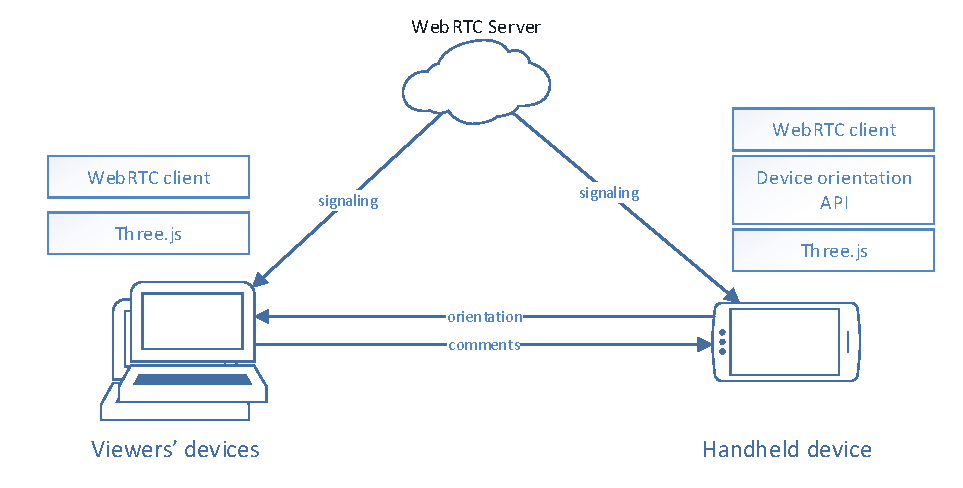
\includegraphics[width=3in]{images/mgia16/system}
  \caption{System architecture based on WebRTC}
	\label{fig:mgia16:system}
\end{figure}

The prototype was built on top of AppRTC\footnote{https://apprtc.appspot.com/} which hosts a website that enables people to start a video conferencing session on the web. To support AR visualization of comments, we utilized the AppRTC code to track device orientation by listening to the device sensors. The AppRTC application is written in Python for the backend and Javascript for the front-end. It takes advantage of being hosted on AppSpot so that it complies with the WebRTC requirements for HTTPS. The AppRTC system allows users to communicate with each other over the Internet. In addition to the video stream, we modified the code to transfer the device orientation data to the receivers' devices via DataChannel. To render comments in the AR visualization, we used the Three.js library\footnote{http://threejs.org/}. The AR visualization is implemented with two graphical layers. The background layer shows the video stream captured by the camera on the mobile device. On top of the background, comments are drawn on the front layer using orientation tracking information to show them in a body-stabilized manner \cite{Billinghurst1998}. 

\subsection{Implementation}

The application starts by turning on the back camera on the mobile device. It then asks the user to enter a “room number” to start the connection. Once this is entered, the application will start a call mode, waiting for other participants to enter the same the room number. Once the call is established, the mobile device will start streaming video and device orientation data to the viewing PC. 

Both users can send comments to each other by clicking on any part of the shared video. The system then calculates the 3D position of the comment in the AR space and waits for the comment text to be entered. Once the user enters the message, the text is displayed on both the sender's and receiver's screens. The motion data of the sender's device is also shared so that the receiver will see the comment appearing at the same place as the sender turns his/her device. 

Three different ways of showing comments on the live video stream were implemented. A list view where the comments are listed on the side of the camera feed view. An AR implementation (AR) where the comments were overlaid on top of the video feed and rotated around the user based on phone orientation, so the comments appear fixed at the location on the video where they were first entered. Finally, an AR + list implementation combined the list view with the AR view. In the next section, we report on a user study exploring these three implementations.

\begin{figure}[ht]
  \centering
  \includegraphics[width=3in]{images/mgia16/participant2}
  \caption{Comment appearing on top of the shared video}
	\label{comments}
\end{figure}


\subsection{User Study}

We conducted a controlled within-subjects user experiment to test the different user interfaces for displaying comments. There were three conditions: L) comments in a list, AR) comments on the video with AR visualization, and L+AR) comments on both. The experiment started with the participants giving consent and answering questions about demographic information. Then they went through a training session to get familiar with the application and the experimental procedures.

To simulate different environments for the user, we used 180-degree panoramic images projected around the user on large screens to simulate different real spaces (see Figure \ref{fig:mgia16:participant}). We selected four different images where the user might be interested in sharing his or her surroundings, varying in terms of indoors/outdoors and busy/quietness. A different background was randomly assigned for each condition between subjects. 

\begin{figure}[ht]
  \centering
  \includegraphics[width=3in]{images/mgia16/participant1}
  \caption{Participant during the experiment}
	\label{fig:mgia16:participant}
\end{figure}

Each participant was asked to sit in the middle of the projection screens showing the background image, hold a smart phone, and aim its camera at the background to share it with remote users. The experimenter simulated multiple users sending comments on the shared video in a ‘Wizard of Oz' style setup. There were six predefined comments for each background. The comments appeared on the screen in three different styles depending on the experimental condition. The order of the conditions was counterbalanced using a balanced Latin square design. While watching the comments, the participant was asked to remember which part of the background each comment was talking about and who made the comment, which could be identified by the colour of the comment. There were up to four colours (commenters) in the experiment. The comments faded away one minute after being displayed. This was to simulate the user receiving multiple comments while having limited time to read them all.


After completing a condition, participants were asked to place a printed version of each comment on a background image, at the correct location, and with the correct colour, testing their knowledge of where each comment appeared. The participants were also requested to answer a questionnaire on system usability \cite{brooke1996sus} and social presence \cite{Harms2004}. The questions were slightly modified to fit the scenario being tested and only focused on one-way communication. Table \ref{table:social_questions} shows the social presence questions that were answered on a seven-level Likert scale rating (1: strongly disagree - 7; strongly agree). 

\begin{table}[h]
  \centering
  \caption{Social presence questionnaire. Negative questions marked with (-)}
  \label{table:social_questions}
  \begin{tabular}{lll}
    Q1 & Comments from others were clear to me.          \\
    Q2 & It was easy to understand comments from others. \\
    Q3 (-) & Understanding others' comments was difficult.  \\
    Q4 & I could tell how others felt by my video sharing.\\
    Q5 (-) & Others' emotions were not clear to me.\\
    Q6 & I could describe others' feelings accurately.
  \end{tabular}
\end{table}

% [do you want to show system usability questions as well?]

After finishing all three conditions, participants answered a post-experiment questionnaire that asked them to rank and compare all three conditions in terms of strengths and weaknesses. Finally, the experiment ended with a debriefing and the opportunity for participants to provide open-ended comments.

\subsection{Results}

We recruited 20 participants (11 female, aged between 19 and 35 years old, Median=27.5, SD=4.55). Most (95\%) of them had experience with live video streaming a few times a week to a few times per month and 80\% were familiar with AR applications. We used a non-parametric Friedman test for all the results with alpha=0.05, and post-hoc tests using Wilcoxon signed-rank tests with the Bonferroni correction (alpha=0.017)

The statistical result for SUS (see Figure \ref{fig:mgia16:questions_sus}) showed that there was a statistically significant difference between conditions ($X^2(2)=9.658, p=0.008$). Post-hoc analysis showed significant differences between L and AR (Z=-2.638, p=0.008) and between L and L+AR (Z=-2.559, p=0.010). However, there was no statistically significant differences between AR and L+AR (Z=-0.197, p=0.844). This shows that the list condition on its own was considered considerably less usable than the other two conditions.


\begin{figure}[ht]
  \centering
  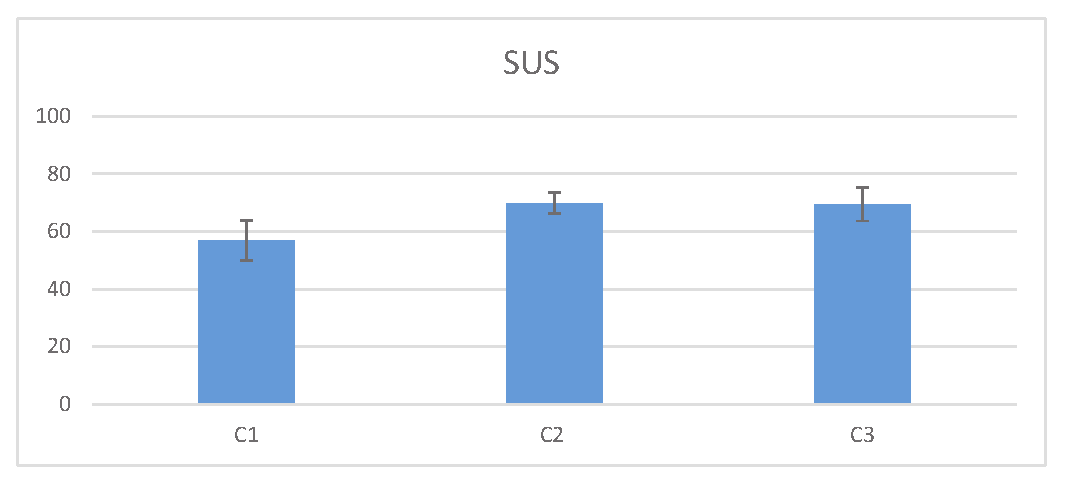
\includegraphics[width=2.5in]{images/mgia16/sus.eps}
  \caption{SUS score}
  \label{fig:mgia16:questions_sus}
\end{figure}

As for the social presence questions (see Figure \ref{fig:mgia16:social_presence}), we inverted the responses on the negative questions Q3 and Q5, to allow all questions to be aggregated, combining the answers for both perceived message understanding and affective understanding. There was a statistically significant difference in perceived social presence ($X^2(2)=16.892, p<0.001$). Post-hoc analysis found there were significant differences between L and AR (Z=-3.459, p=0.001) and between L and L+AR (Z=-3.311, p=0.001) while there was no statistically significant difference between AR and L+AR (Z=-0.427, p=0.670). This shows that the list condition (L) was perceived as being less easy to understand, and that viewer comments in this condition were less clear.

\begin{figure}[ht]
  \centering
  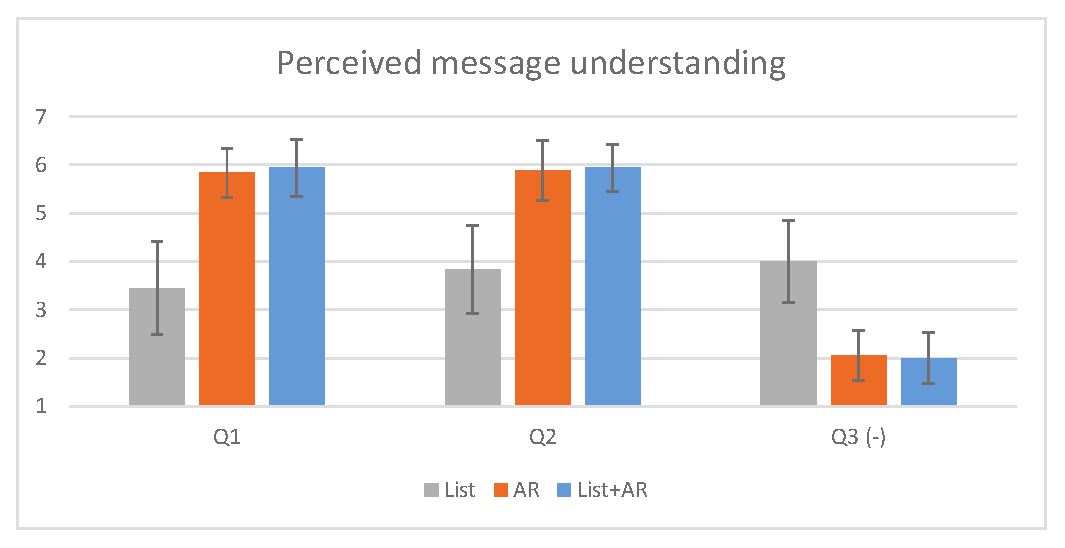
\includegraphics[width=2.5in]{images/mgia16/message.eps}
  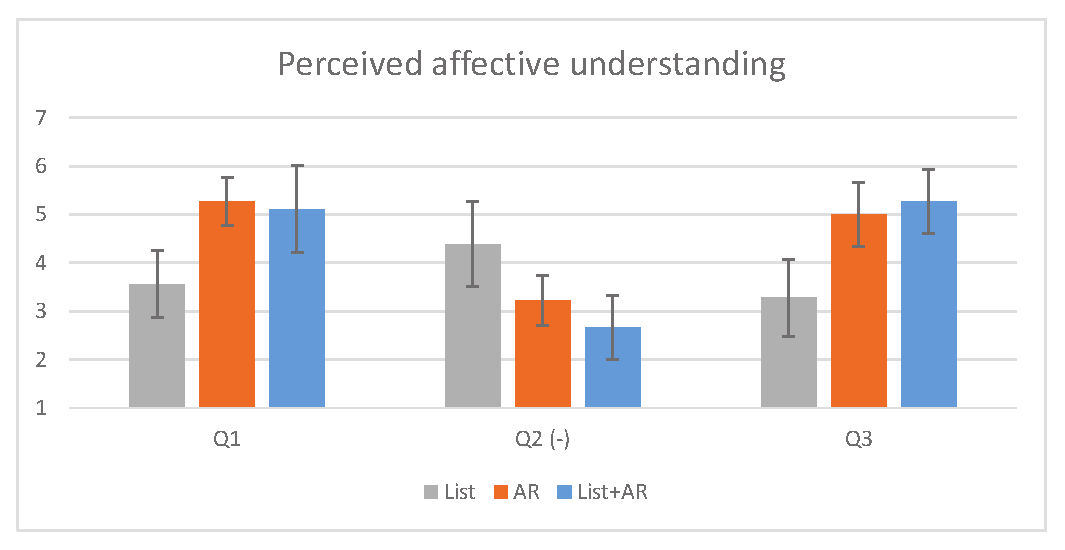
\includegraphics[width=2.5in]{images/mgia16/affective.eps}
  \caption{Results for the social presence questions "perceived message understanding" and "perceived affective understanding"}
	\label{fig:mgia16:social_presence}
\end{figure}

As for the ranking results (see Figure \ref{fig:mgia16:ranking}), we calculated the average of the answers (where 3=highest ranking, 1=lowest ranking). The results show a statistically significant difference between conditions ($X^2(2)=9.100, p=0.011$). Post-hoc analysis showed a significance level set at $alpha$=0.017. There were significant differences between L and AR (Z=-2.766, p=0.006) and between L and L+AR (Z=-2.502, p=0.012). However, there was no statistically significant difference between AR and L+AR (Z=-0.039, p=0.969). This shows that the list condition (L) was ranked the worst out of the three conditions.

\begin{figure}[ht]
  \centering
  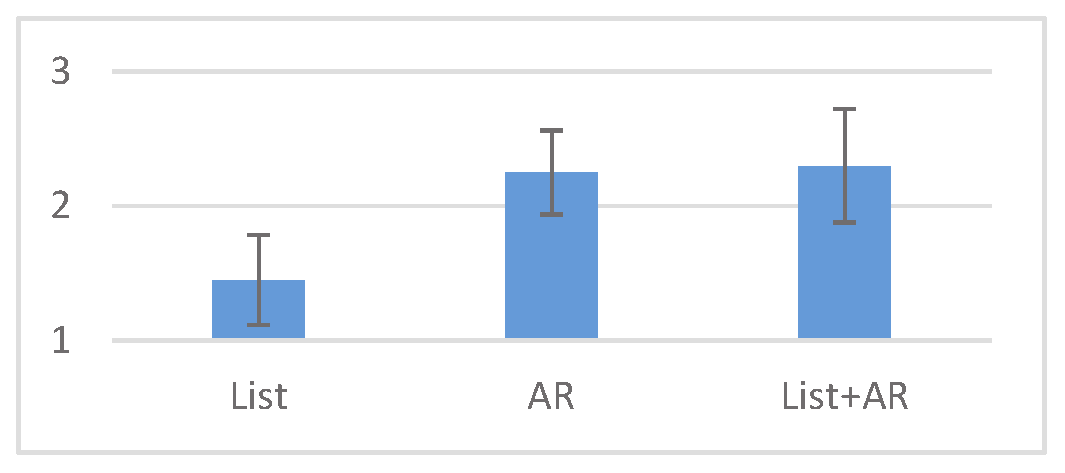
\includegraphics[width=2.5in]{images/mgia16/ranking.eps}
  \caption{Results for conditions ranking questions}
	\label{fig:mgia16:ranking}
\end{figure}

For the task of matching the position and colour of the comments (see Figure \ref{fig:mgia16:questions_matching}), The results show that there was a statistically significant difference ($X2(2)=22.030, p<0.001$). Post-hoc analysis showed that there was no significant difference between the L and AR conditions (Z=-1.016, p=0.310). However, there was a statistically significant difference between L and L+AR (Z=-3.628, p$<$.001) and between AR and L+AR (Z=-3.447, p=0.001).

\begin{figure}[ht]
  \centering
  \includegraphics[width=2.5in]{images/mgia16/matching.eps}
  \caption{Results for correctly matching comments with background and colour.}
	\label{fig:mgia16:questions_matching}
\end{figure}

Participants were asked free-form questions to comment on their experience in terms of the strengths and the weaknesses of each condition. Approximately 80\% of feedback from the participants noted that in the list condition (L) it was more difficult to identify the area of the comments comparing to the AR conditions. Eight participants (40\%) found it more challenging to remember the comment colours as a means to identify the person who sent the comment. 

In the AR and L+AR conditions participants felt that the comments were contextual and relevant to the background. For example, \textit{"It's easier to remember comments on video (AR) because the comments acts as cues on the video you can directly see what the people are commenting on which I think makes me feel more connected to them"}. One of the strengths of the L+AR condition commented on included having an overview of the list of comments even if they are outside the current viewpoint of the user. 

However users felt that comments in the L+AR condition could clutter the UI and partially block the background. One participant said \textit{"The screen just became too busy with comments that I don't have the time to actually sort out the comments and associate them on the video"}. Some suggested this could be resolved by making the comments not in the center of view more transparent.
 
We asked the participants what would they like to improve. Most reported that they would like to use a head-mounted display to view comments in the AR mode.  It was also suggested that we use a profile image instead of colours on comments to distinguish remote users.
 
Overall users felt that the AR and L+AR conditions were fun and cool to use, providing comments such as \textit{"It's pretty awesome. I love the experience and I would really like to use this app with my social network."}.


\subsection{Discussion}

From the user study, we found that subjects preferred the conditions that contained an AR view, compared to showing comments only displayed in a list format. They thought these conditions were more usable, provided a higher degree of social presence, and enabled them to better remember the comment layout. This is probably because the spatial association of comments increases the likelihood of the message being understood and being attended to.

We expected that one of the AR conditions (AR or L+AR) would have been more popular than the other, however this was not the case. Some users preferred L+AR over the AR as the former provided an overall list of comments even if they were not visible in the current user viewpoint; making the user more aware of new comments without needing to look around to find them. Other users preferred the AR only condition, as the screen is less crowded. One solution to this might be by hiding the comments on the list that are visible on the AR view, removing any duplication. Alternatively we could use a radar view that shows dots to represent comments. 

We learned more about how to make the live streaming a better experience for the user. Some users found the one-minute timeout for the comments fading away to be too fast. Associating the comments with colour to represent different users may not be the best option. An alternative approach would be to use an avatar or name of the person to identify the comment source. 

The study has a number of limitations that we will have to address in the future. The experiment was conducted in a simulated environment rather than outdoors. We also used a static background image to simplify the conditions. However in real life, things will be moving in the background (i.e. people walking, cars passing by). In such scenarios, the comments in the AR condition may not stick to the moving objects. However, this could be solved by using image processing techniques to track objects that will allow the comment to be moved with them. Finally, the all of the comments were generated by an experimenter and were fixed, rather than coming from real people who could write whatever they liked.    

\subsection{Summary}

In this paper, we investigated AR annotations for social live video streaming. We conducted a user study testing three variations of the interface for showing comments: 1) a list, 2) an AR view and 3) both list and AR views. Participants felt that the AR and the List + AR conditions were significantly better than the List condition in terms of system usability and social presence. This was probably because the spatial alignment of comments increases the likelihood of them being understood and attended to.

In the future, we plan to investigate alternative mechanisms for communicating in a social live video sharing sessions, such as using sketching or emojis. We will also explore how depth cameras could be integrated into the system to enrich the social sharing experience by providing improved tracking and environment recognition. Finally, we would like to conduct more extensive user studies that test various user interface designs for using AR for sharing social experiences. This could include being able to navigate back in time to see comments before. 



\section{AR Annotation using 3D sensors}
\label{sec:3D}

% =============== PREVIOUS WORK ================

% A. Nassani, H. Bai, G. Lee, and M. Billinghurst, “Tag it!: AR annotation using wearable sensors,” in SIGGRAPH ASIA 2015 Mobile Graphics and Interactive Applications on - SA '15, 2015, pp. 1–4.

% A. Nassani, H. Bai, G. Lee, and M. Billinghurst, “Extending HMD by chest-worn 3D camera for AR annotation,” in SIGGRAPH ASIA 2015 Mobile Graphics and Interactive Applications on - SA '15, 2015, no. Figure 2, pp. 1–2.

% =============== PREVIOUS WORK ================


% \subsection{abstract}

In this work we describe a wearable system that allows people to place and interact with 3D virtual tags placed around them. This uses two wearable technologies: a head-worn wearable computer (Google Glass) and a chest-worn depth sensor (Tango). The Google Glass is used to generate and display virtual information to the user, while the Tango is used to provide robust indoor position tracking for the Glass. The Tango enables spatial awareness of the surrounding world using various motion sensors including 3D depth sensing, an accelerometer and a motion tracking camera. Using these systems together allows users to create a virtual tag via voice input and then register this tag to a physical object or position in 3D space as an augmented annotation. We describe the design and implementation of the system, user feedback,  research implications, and directions for future work.  


% \subsection{Introduction}


% In our research we are interested in allowing people to place virtual tags at points or objects of interest in their physical world. Recent developments in wearable computing have made this possible by integrating sensing, interaction and display technologies into small body-worn devices. Compared with traditional mobile devices, state-of-the-art wearable devices provide novel interfaces to work with the augmented digital contents, and make the Augmented Reality (AR) applications more natural and intuitive to use. For example, the head-worn Google Glass\footnote{	http://www.google.com/glass/start/} allows people to interact using their voice and head movements while freeing their hands for other tasks. Moreover,the Tango \footnote{https://www.google.com/atap/project-tango/} offers the capability of spatial awareness through tracking the 3D position of the device using a depth-sensing camera. It provides the Visual Inertial Odometry (VIO) data that gives the user's global position and orientation in 3D space to assist them to interact with virtual objects registered in the real world in a more immersive way.

% We are interested in combining various wearable technologies to enhance the AR experience. We investigate a scenario where the user wears Glass together with the Tango mounted on their chest to create and review 3D augmented annotations indoors (see Figure\ref{system}). The process of creating AR annotations using the 3D sensor is separate from viewing AR annotation using a head-mounted display (HMD). For example, users' have to turn their body to face the AR tag during creation, however for viewing the AR tags, the user can turn their head to explore the surrounding environment, separate from where their body is facing. The benefit is that it makes the user very natural and comfortable.

% \begin{figure}[ht]
%   \centering
%   \includegraphics[width=\linewidth]{images/mgia16/sampleteaser-01}
%    \caption{AR annotation application scenario. (a) The user is wearing Google Glass on her head and a Tango device on her chest; (b) A sample indoor environment for spatial tagging; (c) The corresponding depth and VIO data from the Tango sensors; (d) The AR view through the Glass display: a virtual tag is now attached a real location on the table.}
%   \label{system}
% \end{figure}

% \subsection{Related Work}

% There have been a number of examples of AR annotation demonstration on mobile devices. For example, mobile AR browsers (e.g. Wikitude or Junaio) can overlay AR tags in the real world using  GPS and other motions sensors. While they were successful with demonstrating the concept of visualizing AR annotation, the registration of virtual objects in the real world can be inaccurate and they can only be used in outdoor large-scale environments. Mobile AR browsers usually create AR tags in advance, but recent research projects have investigated in-situ and interactive creation of AR tags. Kim et al. \cite{Kim:2011:IAS} presented an interactive method where the user stands in a fixed position to calibrate the room model with the gyroscope data. The user can then touch and annotate locations with a rectangle where virtual content, like text, image and 3D models, can be overlaid.  Langlotz et al. \cite{Langlotz:2012:OCP} developed a vision-based orientation tracking system to locate and visualize annotations with pixel accuracy on a real-time generated panorama. Both these systems assume pure rotation from the devices while the user has to stand at the same position while doing the annotation, which dramatically reduces the user experience.

% Meanwhile, a variety of AR annotation methods with wearable interfaces have been presented as well. Sixsense \cite{Mistry:2009:WWU} used a wearable gestural interface for AR annotation. It consists of a camera and a small projector mounted on a hat or coupled in a pendant. The camera tracks user hand gestures and the projector visually augments virtual content on the physical objects that the user is interacting with. However it requires planar surfaces in front of the user for accurate projection because of the lacking of a depth sensor. OmniTouch \cite{Harrison:2011:OTW} is a wearable projection system equipped with depth-sensing technology that enables interactive multi-touch applications on different surfaces. Both the depth camera and projector are rigidly mounted to a form-fitting metal frame, which is worn on the shoulders, and secured with a chest strap. This system extended the typical scenarios supported by Sixsense to  users' on-body surfaces or objects held in hands for image projection by using depth sensors. However, the system itself is still bulky and inconvenient to use because of the need to connect to a desktop computer.

Our system overcomes the limitations mentioned above by combining multiple wearable technologies through a wireless network. The system is small and light enough to comfortably wear, allowing for mobility in the physical world, and being available for annotation not only on 2D surfaces but in 3D space. For example, if the user walks closer to or away from the AR tag (e.g. 3D text or models), it will appear bigger or smaller according to the changes in the perspective view. The system combines Google Glass and Google Tango together to provide compelling wearable AR experience. Google Tango is a self-contained handheld device that contains a motion tracking camera, 3D depth sensing a nine axis accelerometer, gyroscope, compass sensors. It has a rear-facing 4MP RGB/infrared camera, a 180-degree field-of-view fisheye rear-facing camera, a 120-degree field-of-view front facing camera, and a 320 x 180 depth sensor. In contrast, Google Glass has no depth sensing capability but combines computing and display in a highly compact form factor. Connecting the two devices enables us to easily prototype future wearable AR interfaces such as what might be possible with Microsoft Hololens\footnote{https://www.microsoft.com/microsoft-hololens/en-us} or other devices.

\subsection{System Design}

The main application scenario for our prototype system is around sharing messages through creating and viewing location-based AR tags registered in a small scale physical environment. The user wearing the system walks into a room and then places AR tags at various places or on objects. The AR tag content is created by using voice input and placed where the user is looking. The AR tags can be meaningful for users, for example, reminding them of something interesting in this space, or sharing the message with other users as a collaborative tool. The system should work in an arbitrary unprepared indoor environment where no previous knowledge about the space is required. 

Traditionally AR tag tracking uses two different approaches at different  ends off the technology spectrum (see Figure\ref{fig:mgia16:spectrum}) based on the level of detailed information required. At one end there is GPS location-based tracking that can be implemented in a light weight HMD such as Glass. On the other end 3D depth sensing cameras incorporated into a hand-held device (HHD) are capable of indoor tracking and localization. The aim of this system is to combine the benefits of a light weight HMD with a self-contained mobile 3D depth tracking offering not only the outdoor GPS based tracking but also vision based indoor tracking  for AR annotation applications. 


\begin{figure}[ht]
  \centering
  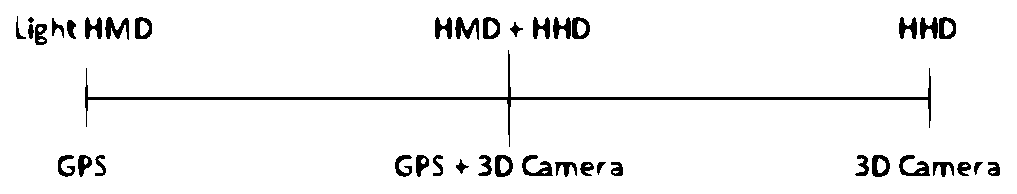
\includegraphics[width=.8\linewidth]{images/mgia16/tango_paper_continuum}
  \caption{The spectrum of AR tag tracking. A head-mounted display with GPS is ideal for outdoor tracking. Hand-held devices (3D camera) can be used for indoor tracking. Glass+Tango enables indoor AR tag tracking on light HMD.}
  \label{fig:mgia16:spectrum}
\end{figure}

\subsection{Implementation}


\begin{figure*}[t]
  \centering
  \includegraphics[width=\linewidth]{images/mgia16/workflow_diagram}
  \caption{System workflow.}
  \label{framework}
\end{figure*}


The system consists of two wearable devices a Google Glass HMD and a Google Tango chest-mounted 3D depth and sensor (see Figure\ref{framework}).

The two devices communicate with each other wirelessly. The Tango extends Glass' sensing ability by sharing the location and pose of the user as well as the tagged target position in the real world. The Glass dynamically overlays virtual tags based on the spatial information received from the Tango, and the background of the Glass display is set to black to act as an optical see through display (see Figure\ref{fig:mgia16:ui}). A white square is displayed on the Glass screen to indicate the center point at which the tango depth camera is facing. The user can initiate the wireless connection by using a three-finger touch gesture on the Glass touchpad, and the AllJoyn library  is used for networking.

Once the system starts on the Tango, it creates a reference coordinate of the surrounding environment. When the user moves, the motion sensor on the Tango will detect the body  position and rotation from the reference origin, both of which are then wirelessly transmitted to the Glass. Combing the head rotation detected by the sensors on the Glass, we can calculate the AR Viewpoint. The position of the AR viewpoint is calculated by adding a measured distance in height from Tango's position to adjust the height difference between the Glass and Tango. The orientation of the AR viewpoint mainly depends on the body's rotation but will be adjusted with the head and body pose difference, if the user turns their head towards a different direction from their chest. 

A speech recognition service is running in the background on the Glass to detect the users' voice input and convert it into text. The text will appear on the upper left corner of the display for for the users confirmation. This function is implemented as an Android service that utilizes Google API for speech recognition and so requires an internet connection. Once the user is satisfied with the recognized text, they can tap on the Glass touchpad while looking where they wish to add the AR tag by using the white square in the display. The Glass sends a request to Tango to identify the location of the AR tag in 3D space.

Combining the AR view point and the recognized text, we can convert the target position (the center point of the depth image indicated by the white square) to the global position relative to the origin. The Tango returns the global position of the AR tag to the Glass. This information is used to construct an AR tag with the speech recognized text that is overlaid on the top of the Glass camera view.

In (Figure\ref{fig:mgia16:ui}), the top left corner shows the last words captured via the voice recognition service, and a white square indicates the center position of Tango's RGB depth frame. The text in the middle of the display "Cup" is an AR tag overlaid on top of a physical cup. 
% * <eng.ala@gmail.com> 2015-06-19T10:04:56.888Z:
%
%  [Somewhere it would be good to mention the tracking accuracy and update speed – how accurate is the Tango position sensing for example]
%

\begin{figure}[ht]
  \centering
  \includegraphics[width=2.5in]{images/mgia16/WIN_20150614_204531_2}
  \caption{View through Glass display of a cup overlaid by an AR tag.}
  \label{fig:mgia16:ui}
\end{figure}


\subsection{User Study }

To evaluate our prototype, we conducted a pilot user study (see Figure\ref{fig:mgia16:scenario}) with ten participants . 4 female, 6 male ranging in age between 23 to 33 years old (\textit{SD= 4.35}). The main focus of the study was to measure the usefulness of the proposed system. Participants were asked to create three different AR tags for three different objects inside the room, with voice input, and then to walk around to observe how well the AR annotation is placed at the selected location. Participants had the freedom to assign any text to any object they wish in the test. The experiment conductor explained the tasks before the experiment and gave examples of target objects and names to use for voice input. All participants completed the tasks within 5 minutes. 

\begin{figure}[ht]
  \centering
  \includegraphics[width=3in]{images/mgia16/axis_lo}
  \caption{User study scenario}
  \label{fig:mgia16:scenario}
\end{figure}

Qualitative feedback about the system was collected from participants including how they would describe their experience using our system, what they liked and didn't like. Questions (Table \ref{table:questions}) were in four categories: (C1) Using the voice commands to create AR tag, (C2) Tap on glass touch panel to attach the AR tag, (C3)  Walk around to find AR tag stick to the original position, (C4) Overall AR tagging experience. In each category we asked the participants the following questions

\begin{table}[ht]
  \centering
	\caption{Survey questions}
    \label{table:questions}
    \begin{tabular}{r l}
    \hline
    Q1 & I found it easy to use \\ \hline
    Q2 & I found it natural to use \\ \hline
    Q3 & I found it physically challenging \\ \hline
    Q4 & I found it mentally challenging \\ \hline
    Q5 & I found it useful \\ \hline
    \end{tabular}
\end{table}

The answers were captured on a Likert scale of 1 to 7 in which 1 is "strongly disagree" and 7 is "strongly agree".

We used the Wilcoxon Signed Rank test on the results to measure significance. Based on the results, we found that participants rated significantly higher than neutral (4) on Q3 (p=.01, .009, .007 and .041) and Q4 (p=.014, .009, .007 and .01) for all categories (C1, C2, C3, C4). Q2 (p=.033) and Q5 (p=.015) were rated significantly higher for category (C3). Q1 for C4 was rated significantly higher (p=.014). (see \ref{survey_results}). The results  for other tasks were rated less significant than neutral level (4). Participants rated the task of walking around the environment was useful with average score of 5.2 out of 7 as well as being not mentally challenging with an average score of 2 out of 7. This highlights the usefulness of the system in assigning AR tags and recognizing them when they appear on their display while walking around the environment. 

In addition to the survey, we also asked participants open questions to comment on the system usability. A total of 3 out of 5 participants mentioned that they would use this system for virtual sticky notes, and they also provided some positive feedback such as "the system could be useful for finding a meeting room or a colleague's desk in an open plan area". There were also a few suggestions for improving the system, such as "allow the user to manually adjust the location of the AR tag" or "integrate with eye tracking to assist placing the AR tag within the field of view ". Participants appreciated  the concept of wirelessly connecting depth camera to a wearable HMD to enable the 3D spatial tracking.    


\begin{figure}[ht]
  \centering
  \includegraphics[width=\linewidth]{images/mgia16/user_study_results2}
  \caption{Average results of survey questions. Bars indicate standard error. *=statistically significant}
	\label{survey_results}
\end{figure}


\subsection{Discussion}

% * <eng.ala@gmail.com> 2015-06-19T10:05:25.941Z:
%
%  It would be good to add some more comments about why you got the results that you did
%
While our prototype  system demonstrates the concept of harmonizing the use of multiple wearable devices for AR visualization, there are few limitations in the current implementation of the system. It was observed that some users had difficulties with voice input as they were not native English speakers, which made the participants use several attempts before the intended word was correctly recognized.  

The current system tracks the 3D environment relative to the starting position, which requires the users to start the system at the same position and orientation in each test trail to keep the annotation in place between uses for sharing. This could be overcome in the future by storing the reconstructed 3D map of the environment and reusing it instead of generating it from scratch every time. 

\subsection{Future Application Scenarios}

Many implementation scenarios could benefit from combining a light head-mounted display with a chest worn 3D depth camera,  such as 1) Navigation, 2) Remote collaboration and 3) Social sharing. In this section we describe each of these in more detail.

Navigation is a scenario where this system can be useful. The user could navigate in an outdoor environment using GPS on Glass or similar smart glass display. Google Glass, being an unobtrusive head-mounted display, allows for hands-free navigation. However when the user enters a building, the GPS stops working and the system switches to indoor navigation using the 3D depth camera of the Google Tango device. Combining two devices enables seamless transition during a navigation experience. For example, a person could be shopping to find a particular item and use outdoor GPS tracking to guide them to the store. Once inside the store the Tango depth sensing hardware can help with navigating to find the particular product on the shelf.

Remote collaboration is another scenario where this application could be useful. A local user could transmit reconstructed 3D geometry of the environment using the Tango device to the remote user. The remote user will then have a more detailed view of the environment comparing to 2D sharing such as with a video stream. With the 3D geometry of the environment, the remote user can view the scene from different angles that helps provide better understanding of the surroundings of the local user. Placing AR tags in a 3D environment helps maintain the location of the AR tag especially when the viewing perspective is changed to the point from when it was original recorded

An additional use of the system could be in a social sharing experience where multiple users of the system could collaborate to add, edit and manipulate AR tags in the shared environment. 
% * <eng.ala@gmail.com> 2015-06-19T10:02:27.344Z:
%
%  put more information
%

\subsection{Summary}

This section presented a wearable AR system combining tracking technologies to provide a compelling indoor AR experience for spatial annotation application. By wearing the system, users can create virtual tags with text content generated by voice input and place it where they are looking at. The virtual tags can be visualized in place as a reminder for the users.  

Different scenarios can be implemented and tested based on the prototype with multi wearable devices. There are also a number of ways this research could be extended. In the future, we would like to further develop our efforts in designing interaction scenarios for our system, such as wearable gaming or collaboration. We also plan to develop the system further to expand the use of chest worn device for various interaction techniques (e.g. gesture recognition).


\input{Chapters/43-pano}
